% !TEX TS-program = XeLaTeX
\documentclass[a4paper]{article}


% https://tex.stackexchange.com/a/5365
% Must
\usepackage[table]{xcolor}

\usepackage{tabularx}


\usepackage{tikz}
\usepackage{fontspec,lipsum}
%\usepackage{color}


% https://tex.stackexchange.com/questions/172234/define-and-set-length-in-one-command
\newcommand{\deflen}[2]{%      
    \expandafter\newlength\csname #1\endcsname
    \expandafter\setlength\csname #1\endcsname{#2}%
}

\newcommand{\goldenratio}{1.618}

% Page margins
\deflen{horizontalmarg}{1.0cm}
\deflen{verticalmarg}{\dimexpr(\goldenratio\horizontalmarg)}

\usepackage[top=\the\verticalmarg, bottom=\the\verticalmarg, 
  left=\the\horizontalmarg, right=\the\horizontalmarg]{geometry}


\deflen{lowerbaroffset}{0.8cm}

\deflen{contentswidth}{\dimexpr(\paperwidth-2\horizontalmarg)}
\deflen{contentsheight}{\dimexpr(\paperheight-2.01\verticalmarg)}

\deflen{halfwidth}{\dimexpr(0.5\contentswidth)}


\deflen{paramarg}{0.5cm}

\deflen{colwidth}{\dimexpr(\halfwidth-\paramarg)}

\deflen{lowersectionstart}{\dimexpr(0.5\contentsheight)}
\deflen{headermarg}{2cm}

%% The vertical lines at which things should align
\deflen{haligni}{0cm}
\deflen{halignii}{\colwidth}
\deflen{haligniii}{\dimexpr(\halfwidth+\paramarg)}
\deflen{haligniv}{\dimexpr(\contentswidth)}


%% Horizontal lines at which things should align
\deflen{valigni}{\contentsheight}
\deflen{valignii}{\dimexpr(\contentsheight-\headermarg)}
\deflen{valigniii}{\lowersectionstart}
\deflen{valigniv}{\dimexpr(\lowersectionstart-\headermarg)}


% A paragraph: Args (X, Y, text)
\newcommand{\anemoparagraph}[3]{
  \node[anchor=north west,style={inner sep=0,outer sep=0}] at (#1,#2) {
    \begin{minipage}[l]{\the\colwidth}
      #3
    \end{minipage}
  };
}

% Draw a vertical bar across the contents area
\newcommand{\vhelper}[1]{\draw[color=gray] (#1,0cm) -- (#1,\the\contentsheight);}

% Draw a horizontal bar across the contents area
\newcommand{\hhelper}[1]{\draw[color=gray] (0cm,#1) -- (\the\contentswidth,#1);}

% Display helper lines
\newcommand{\helpers}{
  \draw[color=gray] (0,0) rectangle (\the\contentswidth, \the\contentsheight);
  \vhelper{\the\halignii}
  \vhelper{\the\haligniii}
  \hhelper{\the\valignii}
  \hhelper{\the\valigniii}
  \hhelper{\the\valigniv}
}

% A4: 21.0 × 29.7
\pagenumbering{gobble}
\setmainfont[Path=../fonts/]{Muli-Regular.ttf}

% (x, y, contents)
\newcommand{\mainheader}[3]{
  \setmainfont[Path=../fonts/]{BoingBold.otf}
  \node[anchor=north west] at (#1,#2) {\Huge #3};
  \setmainfont[Path=../fonts/]{Muli-Regular.ttf}
}



\definecolor{Anemored}{RGB}{255, 33, 63}


% https://tex.stackexchange.com/a/159576
\newcommand{\HRule}[1][\medskipamount]{\par
  \vspace*{\dimexpr-\parskip-\baselineskip+#1}
  \noindent\rule{\linewidth}{0.2mm}\par
  \vspace*{\dimexpr-\parskip-.5\baselineskip+#1}}

% To be used inside a column
% contents
\newcommand{\subheader}[1]{
  \color{Anemored}
  \begin{flushleft}
    \Large #1
  \end{flushleft}
  %\noindent\rule{\the\colwidth}{0.4pt}
  \HRule[0cm]
  \vspace{0.5cm}
  \color{black}
}


% A two-column table suitable for specs
\newcommand{\spectable}[1]{
  \begin{tabularx}{\colwidth}{X X}
    #1
  \end{tabularx}
}

% TODO: See if Melissa provided some design document
% with precise specs of margins, font sizes, etc.

\begin{document}
\rowcolors{2}{gray!25}{white}
\noindent
\begin{tikzpicture}[x=1cm, y=1cm]
\definecolor{anemored}{rgb} {1.00,0.129,0.247}
\helpers

\mainheader{\the\haligni}{\the\valigni}{Anemobox Product Description}
\anemoparagraph{\the\haligni}{\the\valignii}{
  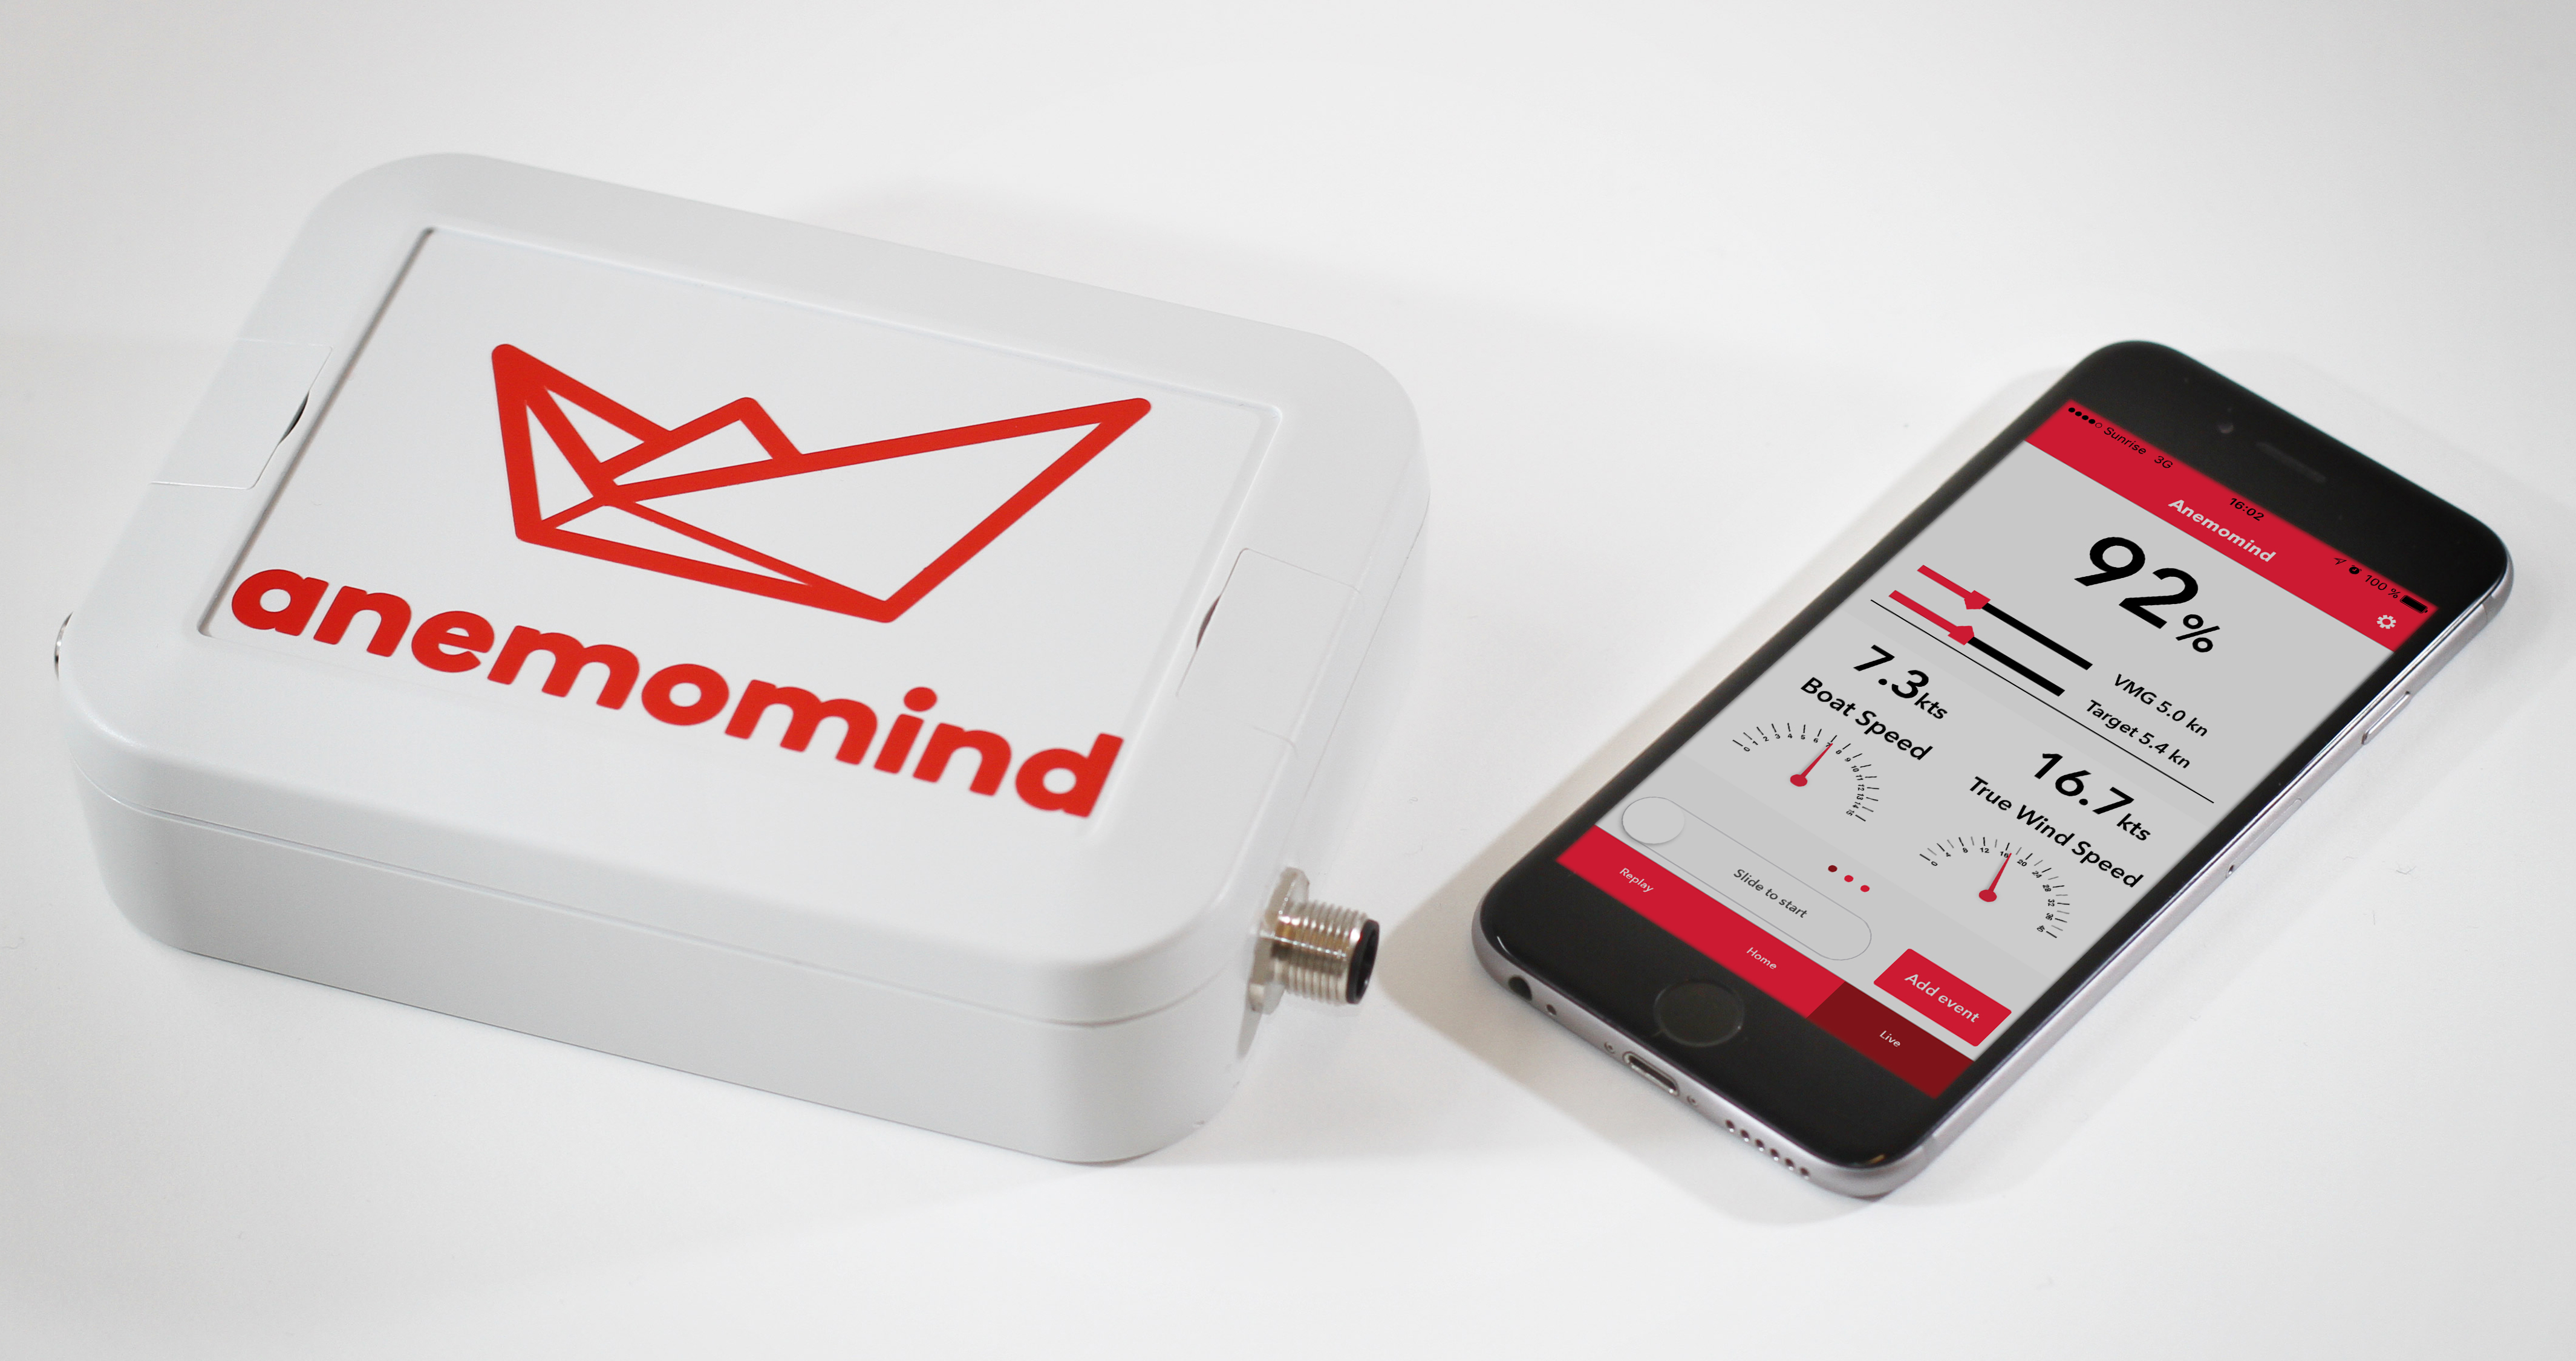
\includegraphics[width=\the\colwidth]{../images/anemobox10.jpg}
  \subheader{Minimum requirements}
  To use the Anemobox, you need at least
  \begin{itemize}
    \item A boat equipped with an NMEA2000/NMEA0183 wind sensor
    \item An iOS device, such as iPad or iPhone
    \item 9-24 Volts DC power supply
  \end{itemize}
}
\anemoparagraph{\the\haligniii}{\the\valignii}{
  \tiny
  \subheader{Features}
  {
  \begin{itemize}
    \item Auto calibrated true wind computation
    \item Boat performance computation
    \item Wireless connectivity Bluetooth 4.0 and WiFi
    \item Data logging with automatic cloud sync
    \item Waterproof
    \item NMEA 0183 and 2000 input/output
    \item 10Hz satellite positioning (GPS, GLONASS and BeiDou)
  \end{itemize}
  }
  \subheader{Specs}
  \spectable{
    GPS networks & multi-GNSS (GPS/QZSS, GLONASS and BeiDou) \\
    GPS networks & multi-GNSS (GPS/QZSS, GLONASS and BeiDou) \\
    GPS networks & multi-GNSS (GPS/QZSS, GLONASS and BeiDou) \\
  }
  
}

\mainheader{\the\haligni}{\the\valigniii}{Order Form}

%

%% \foreach \bound in {north,south,west,east,45} {
%%       \node[anchor=\bound] at (current page.\bound) {I am \bound-bound...};
%%   }
  %\node[anchor=north west, color=anemored] at (0, \the\contentsheight) {\Large Specifications!};
  %\draw[color=anemored, line width=0.25mm] (0, \the\dimexpr(\contentsheight-\lowerbaroffset)) -- (\the\localpwidth, \the\dimexpr(\contentsheight-\lowerbaroffset));
%\node[draw=none] at (0,0) {some text};
%\node[draw] at (0,0) {some text};

\end{tikzpicture}
\end{document} 

